\chapter{Introducción}\label{intro}

%\section{Introducción}

%manipulacion y objetos desconocidos


Hoy en día los robots manipuladores representan una considerable fuerza de trabajo, en la industria por lo general se predefinen rutinas para el robot y este las ejecuta cuando se le ordena, realizando sus tareas con velocidad y precisión.

%CORREGIR TODO EL PRIMER CAPITULO
Actualmente el siguiente paso es la autonomía de los robots, esta autonomía es necesaria para varias aplicaciones: robots de servicio asistencia, exploración, y es útil en toda situación para evitar errores, pero hay varios problemas para lograr esta autonomía, %y el mas ovbio es que hacer en situaciones que desconocidas, como saber que lo esta haciendo bien y como resolver el problema mismo.
uno de los problemas mas comunes es el de los objetos desconocidos.

Sujetar es una de las tareas mas básicas en la robótica, por lo que es completamente necesaria para tareas de mayor complejidad tener una sujetar correcto, para poder tener una sujeción exitosa se necesita tener información especifica acerca del objeto, lo mas común es la posición, las dimensiones, el peso y los puntos de agarre, pero para esto se necesitaría conocer al objeto previamente, en el caso de los objetos nuevos o desconocidos esta información no esta presente, por lo que la sujeción se complica, esto es porque esos datos son importantes y deben ser conseguidos.


Han habido varias obras en esta tarea, ya que es una de las más comunes, algunas obras se enumeran en las compilaciones \cite{carlos2013survey}, como se puede ver en esas obras el uso de un sistema de visión es algo común. Por un largo tiempo, al principio no era tan recomendable como la velocidad de fotogramas y los algoritmos, eran lentos, como se comenta en [3], ahora con cámaras RGBD es más fácil de trabajar con el sensor profundidad de la misma manera que usamos un cámara de color, esto ha sido útil porque es más fácil trabajar el algoritmo de visión en la imagen RGB y la imagen profundidad. \\
%Una de las obras que estamos utilizando como referencia [4] utiliza un sistema de visión hipotético para conocer la posición y algunas otras propiedades del objeto, en nuestro caso utilizamos un sensor ultrasónico para estimar estas propiedades como en algunas obras anteriores [6] de Este laboratorio. \\
%Un objeto puede tener un número infinito de puntos de agarre, para elegir hay una necesidad de tener hipótesis, el que vamos a utilizar se basa en la forma en que los seres humanos captar un objeto, similar al trabajo [7] en el que había resultados basados ​​en la neurociencia Que demostró que un ser humano no usa todo el DOF de su mano, con esto el DOF de manos podría ser reducido, para ajustarse a lo que se llamaba eigengrasps, que eran pre-agarrar posturas. En el trabajo [8] usan una representación de objetos de punto de nube y luego usan ejemplos de agarre humano para tener algún conocimiento empírico para el agarre.
El control que vamos a utilizar se propone en [5], este control de la regla difusa regla emulada (FREN), es un muy simple y fácil de configurar, vamos a utilizar a causa de su parte adaptable. \\

Existen varias formas de clasificar la sujeción, una puede ser; por la información que se tenga del objeto, en esta se clasifica al objeto como conocido, familiar y desconocido, esto puede verse en \cite{bohg2014data,el20113d,carlos2013survey,zaharescuobject}.

Cuando hay suficiente información para realizar la tarea deseada el objeto es clasificado como conocido.

Un objeto familiar es aquel que, aun cuando no se conoce específicamente, comparte características con un objeto conocido. Por otro lado, un objeto desconocido es aquel que no tiene ninguna información previa. \\

El problema del objeto desconocido puede describirse como la falta de conocimiento de cualquier característica importante del objeto, este problema ha sido abordado de diferentes maneras, como tener un escaneo del objeto, usar el contexto en el que se esta trabajando para discriminar otros objetos o una segmentación del fondo para facilitar el reconocimiento.

Este problema se puede dividir en dos partes principales: la segmentación de este objeto y el agarre. En ambos la parte más importante es conseguir tanta información como sea posible. La adquisición de dicha información es posible a través de sensores, pero elegir el sensor a utilizar puede ser difícil para una amplia gama de objetos, ya que algunos podrían no ser detectables por dicho sensor. \\

Estos tipos de objetos son especialmente difíciles debido a la completa falta de información desde el punto de vista de la visión artificial. La segmentación de tales objetos es especialmente difícil.

Esto se debe a que en una imagen en color el color y los gradientes del objeto son desconocidos, por lo que el objeto puede considerarse como ruido o irrelevante en algún momento. Para identificar objetos desconocidos en ese punto, sería útil detectar todos los objetos y luego clasificaros. Debido a estas razones, diferentes enfoques se utilizan para hacer frente a este problema, como el uso de contexto o heurística. Los problemas de agarre también se pueden clasificar como datos impulsados y conducidos por tareas.


Los tipo \textit{Data-driven} intentan obtener los datos más posibles, mientras que la tarea impulsada intenta buscar algo que puede ser útil para la tarea. Un ejemplo de la aproximación impulsada por datos al problema de objeto desconocido sería un método que consiste en el uso de un brazo de robot para el objeto \cite{kaneko1994contact}. Otro ejemplo puede ser el uso y la aproximación de los objetos a las formas primitivas para hacer un reconocimiento \cite{fornas2016fitting, felip2009robust, miller2003automatic, huebner2008selection}. Todos estos enfoques tienen sus limitaciones, y no hay un método general para tratar el problema, ya que uno puede ser eficaz en una aplicación, mientras que, en otros, el método no puede ser utilizado.

Este trabajo se divide en la identificación del objeto desconocido y el alcance del objeto. Para la parte de identificación \cite{hosang2016makes} fue útil como referencia en la segmentación. Dos algoritmos se presentan en \cref{ch.vision}, el primero para la segmentación del objeto y el segundo para adquirir la posición y el tamaño del objeto.
Para el alcance del objeto se utilizó el controlador adaptativo (FREN) \cite{fren}, presentado en \cref{ch.fren}, lo cual resulta conveniente para la simplicidad de su inicialización y adaptación rápida.





\section{Objetivos}

\begin{prop}[Objetivos Específicos]
	\item Sujetar un objeto desconocido en un área semi-conocida \label{objesp:1}
\end{prop} 
El interés de este trabajo es la segmentación de un objeto desconocido con la intención de agarrar.

\begin{prop}[Objetivos Particulares]
	\item Encontrar el objeto (cualquier objeto) \label{objpart:1}
	\item Llegar al objeto \label{objpart:2}
	\item Sujetar el objeto \label{objpart:3}
\end{prop} 

%El primer obetivo especifico e
%one of the particular objectives is.... on one hand.... and on the other hand.....



%the second obj shows that ....

%the third is relateed to....


%it is desaired to sojw 


%to achieve this objectivess we have some apoaches and we used this




\section{Hipótesis}
\begin{itemize}
	\item Es posible realizar la sujeción de un objeto sin tener información previa de este con un \textit{Gripper} comercial, usando información de una cámara RGBD
\end{itemize}

\section{Metodología}
\begin{figure}[h]
	\centering
	\includegraphics[width=0.7\linewidth]{visio/visio3/metodologia}
	\caption{}
	\label{fig:metodologia}
\end{figure}

Tal como puede verse en \cref{fig:metodologia} esta tesis es dividida en 3 capítulos principales, los cuales son acerca de visión artificial y como encontrar un objeto cualquiera, el siguiente capitulo es acerca del control del robot, y en el tercero se habla un poco de la sujeción de objetos, estos capítulos están estructurados en una introducción, algunos conceptos básicos, el tema principal del capitulo, los resultados obtenidos en cada fase, y algunas discusiones acerca del capitulo, en el capitulo 5 se presentan los resultados en conjunto y el capitulo 6 trata conclusiones a las que se llegaron y algunas ideas para trabajos futuros.

 
La motivación de este trabajo es observar el desempeño del control FREN en la sujeción de objetos desconocidos

Este control pertenece a la familia de las ANFIS(Sistema Adaptativo de Inferencia Neuro-Difusa ), algunos conceptos necesarios pueden encontrarse en \cref{basesneurodifusas}.

%Al final habra pastel


Abordamos el problema teniendo información del espacio de trabajo. Una de las ventajas de utilizar la imagen
Encontrar objetos es que podemos discriminar los objetos que son
Fuera del espacio de trabajo. Debido a esto, no importa
El fondo de la imagen.
Una inconveniencia de usar este enfoque es la necesidad de tener un espacio de trabajo definido. Esto puede ser un problema en una aplicación real. Otro problema sería que los materiales reflejantes no son reconocible por la cámara, por lo que es difícil generalizar
El uso de esta cámara para cualquier objeto. \\
En este trabajo tenemos algunas suposiciones para simplificar el problema. \\



El control se divide en 2 fases: una para la segmentación y la otra para alcanzar el objeto

Como se muestra en \cref{fig:1}, el control para llegar al objeto se deja como un control de bucle abierto, ya que estamos utilizando la cámara para obtener la posición del objeto, y dejando la posición del robot a un Control Neuro-Difuso, FREN \cite{fren}.

Por otro lado tenemos el control del robot que puede ser visto en \cref{fig:controldiag}. Esto es un control de lazo cercano con un control de FREN. En este caso, la capacidad de adaptación del control ayudará a regular la fuerza de agarre para que sea lo más mínimo posible evitando el deslizamiento.
Definimos un control de seguimiento de errores, en algunas unidades arbitrarias, mientras intenta hacer que el error sea aproximado a cero.% El error se define como la velocidad del deslizamiento.


\begin{figure}[h]%ca do a ingles!!!!!!!!!!!!!!!!!!!!!!!!!!!!!
	\centering
	\includegraphics[width=1\linewidth]{visio/diagram}
	\caption{Diagrama de control para el posicionamiento dl robot}
	\label{fig:1}
\end{figure}


\section{Definición del Problema}




El problema de investigación que se desea estudiar es conseguir que los robots manipuladores puedan realizar la tarea de acercamiento, para eso se decidió usar redes Neuro-Difusas a que estas usan la experiencia humana en forma de reglas “si X entonces Y”, y usan redes neuronales que pueden ignorar algo del ruido de la situación en la que se encuentran.

Un acercamiento similar puede encontrar se en el trabajo [8], en la que se puede apreciar como la transición entre contacto y no contacto, disminuye si no se tuviera una re-alimentación de las posiciones.

siendo que esta tarea es muy común y fácil de hacer para las personas normalmente, los robots aun tienen movimientos 
poco naturales, esto es debido al tiempo de computo, la medición de los sensores, el pre-procesamiento de la señal para eliminar ruido, el procesamiento de la señal si es que se necesitara, como en visión, la entrada de los datos al controlador y el calculo de la dinámica inversa del robot, ademas del tiempo en que responden los actuadores, todo esto hace realmente difícil poder usar un robot en una tarea no preestablecida en tareas que requieren respuestas rápidas.

Una de las razones por las que es importante este problema es tanto en la estética que se tiene los robots,  como en la parte de la transición entre el no-contacto y contacto, en la cual un ser humano normal puede tomar un objeto de suavemente.

Los controles de redes Neuro-Difusas usan las reglas “si... entonces...” , y redes neuronales, ambas necesitan un conocimiento previo de la situación en la que se estará, pero admiten cambios en el ambiente, mientras estos cambios estén contemplados  o no sean muy extremos.

Otra de las principales razones por la que se planea usar este tipo de control es que al no necesitar del modelo del sistema el tiempo de computo disminuye, por desgracia esto las hace menos precisas, por lo que la frecuencia en que se consiguen los datos es importante, una de los problemas importantes que es que se usara una cámara RGBD para identificar el objeto y el efector final, lo cual al tener una baja frecuencia puede hacer mas lento al sistema, lo que es poco deseable, otro detalle es que la frecuencia de la cámara de profundidad tiene una frecuencia distinta a la de la cámara RGB, por lo que es esta planteando como si usarlas por separado, o esperar a tener ambos datos antes de iniciar con el procesamiento, lo mismo se puede decir del sensor de fuerza.

Se plantea realizar los experimentos en un robot cartesiano, con una interfaz en \textbf{MATLAB}, para la el control y la recolección de datos, en un ambiente controlado, se planea que la cámara RGBD este en una posición fija, la posición del objeto es desconocida, pero se plantea que se mantenga inmóvil, la tarea consiste en encontrar el objeto, acercare a el en el menor tiempo posible y bajar la velocidad conforme se acerca, después de manera lenta tomarlo y llevarlo a otra posición, aunque se estableció que el objeto permanezca inmóvil, se plantea hacer que la parte de visión este siendo evaluada continuamente, tanto para ver el avance del robot, como para preparase para un experimento en el que el objeto este en movimiento moderadamente.



\section{Consideraciones}




\begin{prop}[consideraciones]
	%\begin{observations}
	\item  Se tiene un espacio de trabajo semiestructurado. \label{Assumtion:1}
	\item  El objeto es simétrico. \label{Assumtion:2} %and its composed of the same material 
	\item  La cámara se encuentra estática en un lugar y orientación conocido. \label{Assumtion:3}
	\item  No hay mas de un objeto en el área de trabajo. \label{Assumtion:4}
	\item  No tenemos conocimiento previo acerca de la forma, tamaño, peso o coeficiente de fricción.\label{Assumtion:5}
	%\end{observations}
\end{prop} 











\section{Plataforma de pruebas}

\subsection{robot}
La plataforma que estamos usando es un robot cartesiano de 3 DOF visto en la Fig. \ref{fig:dsc9825}, se utiliza un generador de señal para el voltaje de entrada a los motores de corriente continua, estamos utilizando MATLAB como la interfaz entre el sistema de visión, el control y el generador de funciones.

\begin{figure}
	\centering
	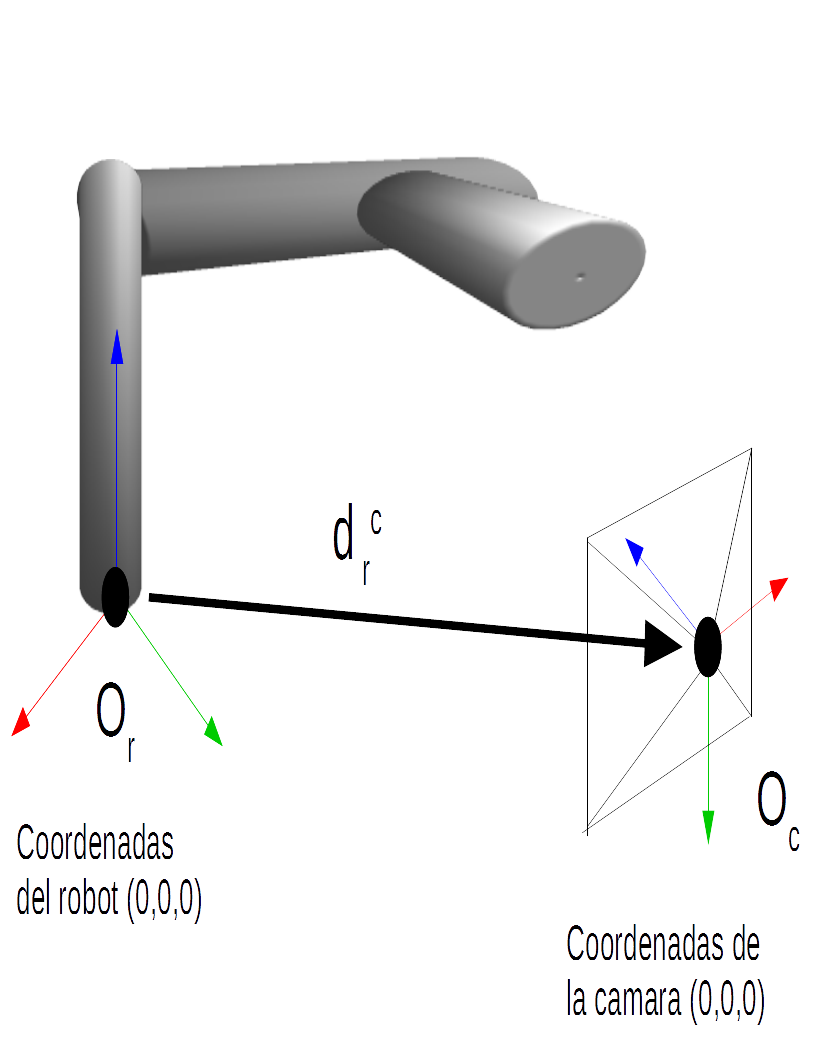
\includegraphics[width=0.5\linewidth]{visio/visio3/coordenadasrobcam2}
	\caption{}
	\label{fig:coordenadasrobcam}
\end{figure}


\begin{figure}
	\centering
	\includegraphics[width=0.5\linewidth]{Imagenes/DSC_9825}
	\caption{}
	\label{fig:dsc9825}
\end{figure}



\subsection{\textit{Gripper}}
El \textit{Gripper} que vamos a utilizar es el modelo SCHUNK WSG-50 que aparece en \cref{fig:dsc9821}, tiene un observador de fuerza, utiliza una fuente de 24V, la abertura es de 10 cm y se puede utilizar con MATLAB para ser operado. \\
Para ser usado se necesitó establecer la comunicación con \textbf{MATLAB}, esta es comunicación básica, en la que se manda un paquete de datos que contiene el comando y las opciones, en el apéndice \ref{codewsg50}, aparece el código que se uso.

\begin{figure}
	\centering
	\includegraphics[width=0.7\linewidth]{Imagenes/DSC_9821}
	\caption{}
	\label{fig:dsc9821}
\end{figure}

\subsubsection{base del \textit{Gripper}}
Se diseño la base para el \textit{Gripper}, y los dedos, se intenta usar el sensor de fuerza y momento, por lo que uno de los 2 dedos tiene una cavidad para este. en el apéndice \ref{label}, se puede encontrar el diseño que se uso.

en la imagen \ref{label}, se encuentra el resultado




\subsection{cámara}

El sistema de visión usa una cámara RGBD que se muestra en la figura \ref{fig:dsc9822}, se uso un programa entre MATLAB y Openni \cite{matlabwrapper}.

La cámara que se uso es el ASUS XTION PRO, su sensor de profundidad tiene un rango operativo de 0,8 metros a 3,5 metros, la resolución de la imagen de color y la imagen de profundidad es $480 \times640$, y la velocidad de fotogramas es 20 cuadros por segundo, ya que es la velocidad de fotogramas del sensor de profundidad. \\

esta cámara trabaja con el software Openni, que es la librería en c++, esta librería tiene funciones para usar la cámara y hacer ciertas operaciones,

al principio se pensaba usar la imagen de rango del sensor de profundidad, que es la distancia desde el sensor hasta el punto censado, esto se pudo evitar gracias a las funciones integradas en Openni.

MATLAB, en ninguna de sus versiones tiene soporte oficial para las cámaras ASUS, aunque si tiene soporte para nuevos dispositivos, pero existe el programa envolvente entre \textbf{MATLAB} y Openni.
el problema con este programa es que requiere de unas condiciones muy especificas para poder ser instalado. entre esas condiciones esta

-usar \textbf{MATLAB} 2010
-compilar con \textbf{Microsoft visual Studio} 2010


una vez instalado se puede usar en otras versiones de \textbf{MATLAB}, en este caso se uso en la versión 2015


\begin{figure}
	\centering
	\includegraphics[width=0.7\linewidth]{Imagenes/DSC_9823}
	\caption{}
	\label{fig:dsc9823}
\end{figure}
\begin{figure}
	\centering
	\includegraphics[width=0.7\linewidth]{Imagenes/DSC_9824}
	\caption{}
	\label{fig:dsc9824}
\end{figure}





%FIGURES